%% ============================================================
%%  Donatien Schmitz — Software Engineer CV
%%  Compile with:  pdflatex engineer-cv.tex
%% ============================================================

\documentclass[9.5pt, a4paper]{article}

\usepackage[a4paper,
  top=0mm, bottom=0mm, left=0mm, right=0mm,
  noheadfoot, nomarginpar]{geometry}

\usepackage{xcolor}
\usepackage{tikz}
\usetikzlibrary{calc}
\usepackage{eso-pic}
\usepackage{enumitem}
\usepackage{hyperref}
\usepackage[T1]{fontenc}
\usepackage[utf8]{inputenc}
\usepackage{helvet}
\renewcommand{\familydefault}{\sfdefault}
\usepackage{graphicx}
\usepackage{microtype}
\usepackage{calc}
\usepackage{eurosym}


% ── Colours ───────────────────────────────────────────────────────────────────
\definecolor{hdr}{HTML}{3a3a3a}
\definecolor{sidebar}{HTML}{ede8e0}
\definecolor{accent}{HTML}{10b981}
\definecolor{dark}{HTML}{1a1a1a}
\definecolor{muted}{HTML}{6b6b6b}
\definecolor{award}{HTML}{854d0e}

\hypersetup{colorlinks=true, urlcolor=accent, linkcolor=accent,
  pdfauthor={Donatien Schmitz}, pdftitle={Donatien Schmitz — CV}}

\pagestyle{empty}
\parindent=0pt
\setlength{\parskip}{0pt}

% ── Layout dimensions ─────────────────────────────────────────────────────────
\newlength{\sideW}  \setlength{\sideW}{0.32\paperwidth}
\newlength{\mainW}  \setlength{\mainW}{0.68\paperwidth}
\newlength{\spad}   \setlength{\spad}{6.5mm}
\newlength{\mpad}   \setlength{\mpad}{8mm}
\newlength{\hdrH}   \setlength{\hdrH}{29mm}

% ── Page backgrounds (header + sidebar) ───────────────────────────────────────
\AddToShipoutPictureBG{%
  \begin{tikzpicture}[remember picture, overlay]
    % Dark header strip
    \fill[hdr] (current page.north west)
      rectangle ([yshift=-\hdrH] current page.north east);
    % Beige sidebar (below header)
    \fill[sidebar]
      ([yshift=-\hdrH] current page.north west)
      rectangle ([xshift=\sideW] current page.south west);
    % Chevron pointing down from sidebar
    \coordinate (chevMid) at ([xshift=0.5*\sideW, yshift=-\hdrH] current page.north west);
    \fill[sidebar]
      ([xshift=-8mm] chevMid) --
      ([yshift=-7mm] chevMid) --
      ([xshift=8mm]  chevMid) -- cycle;
    % Circular photo in header
    \begin{scope}
      \clip ([xshift=0.5*\sideW, yshift=-0.5*\hdrH] current page.north west)
        circle (11.5mm);
      \node at ([xshift=0.5*\sideW, yshift=-0.5*\hdrH] current page.north west)
        {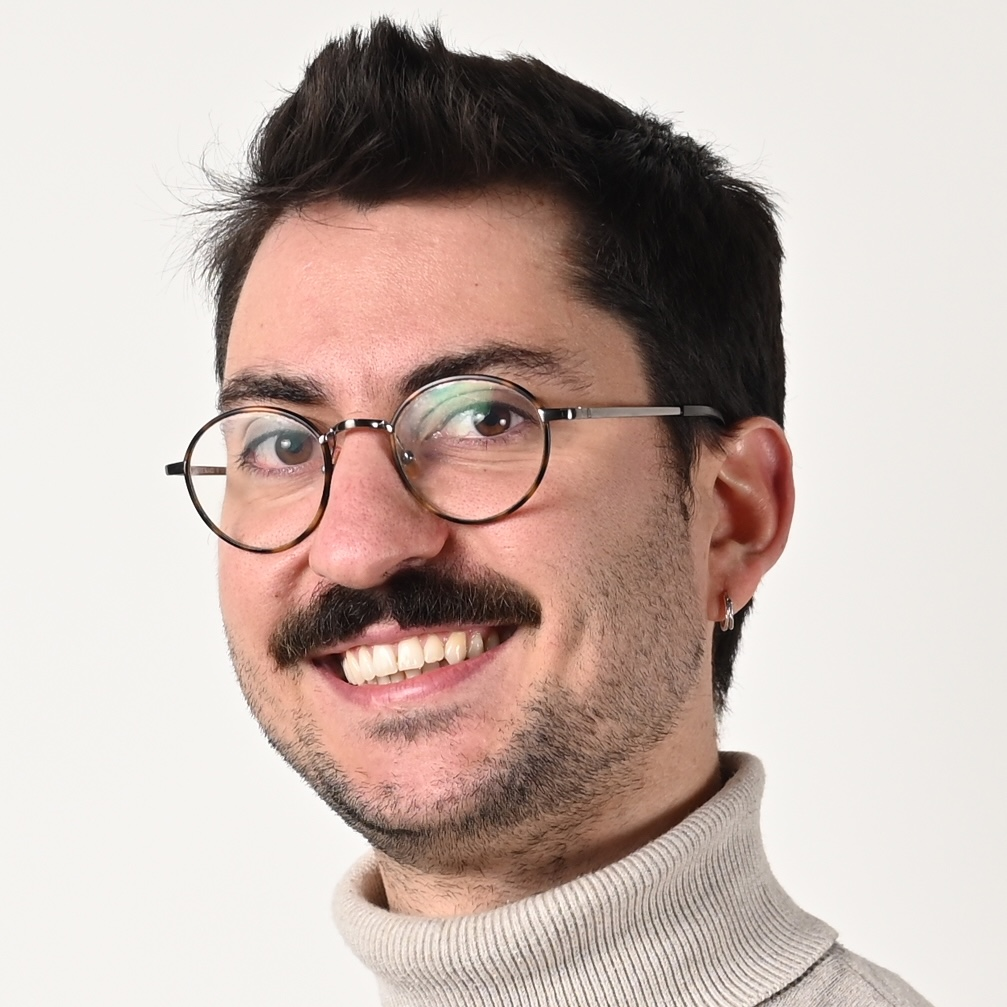
\includegraphics[width=23mm]
          {profile_picture_zoomed.jpeg}};
    \end{scope}
    \draw[accent, line width=1.4pt]
      ([xshift=0.5*\sideW, yshift=-0.5*\hdrH] current page.north west)
      circle (11.5mm);
    % Name in header
    \node[anchor=west, text=white, font=\fontsize{22}{24}\bfseries]
      at ([xshift=\sideW+\mpad, yshift=-0.38*\hdrH] current page.north west)
      {Donatien Schmitz};
    % Title in header
    \node[anchor=west, text=muted!55!white, font=\fontsize{10}{12}\selectfont]
      at ([xshift=\sideW+\mpad, yshift=-0.68*\hdrH] current page.north west)
      {Software Engineer};
  \end{tikzpicture}%
}

% ── Helpers ───────────────────────────────────────────────────────────────────
\newcommand{\sidesec}[1]{%
  \vspace{5pt}%
  {\bfseries\color{dark}\normalsize #1}\par\nopagebreak
  {\color{accent}\rule{\linewidth}{1.2pt}}\par
  \vspace{2pt}%
}

\newcommand{\mainsec}[1]{%
  \vspace{4pt}%
  {\large\bfseries\color{dark} #1}\par\nopagebreak
  {\color{dark!30}\rule{\linewidth}{0.7pt}}\par
  \vspace{2pt}%
}

\newcommand{\jobentry}[4]{%
  {\bfseries\color{dark}\small #2}\par
  {\color{accent}\footnotesize #1}\par
  {\color{muted}\footnotesize #3}\par
  \vspace{1pt}%
  #4%
  \vspace{4pt}%
}

\newcommand{\sideskill}[2]{%
  {\bfseries\color{dark}\small #1}\par
  {\color{muted}\footnotesize #2}\par
  \vspace{3pt}%
}

\newcommand{\ctact}[2]{%
  \noindent
  \begin{tikzpicture}[baseline=-0.5ex]
    \node[circle, fill=accent, inner sep=1.6pt, minimum size=13pt,
          font=\color{white}\fontsize{5}{5}\selectfont] {#1};
  \end{tikzpicture}\hspace{3pt}{\color{muted}\small #2}\par\vspace{3pt}%
}

\newcommand{\award}[1]{\,{\scriptsize\bfseries\color{award}[#1]}}

\setlist[itemize]{
  leftmargin=1.1em, itemsep=1pt, topsep=1pt, parsep=0pt,
  label={\color{accent}\small\textbullet}
}

% ══════════════════════════════════════════════════════════════════════════════
\begin{document}

% Push content below the header
\vspace*{\hdrH}

\noindent
% ─── LEFT SIDEBAR ────────────────────────────────────────────────────────────
\begin{minipage}[t]{\sideW}
\hspace{\spad}\begin{minipage}[t]{\sideW - 2\spad}
\vspace{9mm}

\sidesec{Contact Details}
\ctact{@}{\href{mailto:schmitzdonatien@gmail.com}{schmitzdonatien@gmail.com}}
\ctact{GH}{\href{https://github.com/donaschmi}{github.com/donaschmi}}
\ctact{in}{\href{https://linkedin.com/in/donatien-schmitz-a34039116}{LinkedIn}}
\ctact{$\circ$}{Belgium\,/\,Remote}

\sidesec{Education}

{\bfseries\color{dark}\small PhD CS \& Engineering}\par
{\color{muted}\footnotesize UCLouvain, Belgium}\par
{\color{accent}\footnotesize 2021 – 2026}\par
{\color{muted}\footnotesize\textit{Resource Mgmt in Distributed\\Stream Processing}}\par
\vspace{5pt}

{\bfseries\color{dark}\small Master Computer Science}\par
{\color{muted}\footnotesize UCLouvain, Belgium}\par
{\color{accent}\footnotesize 2019 – 2021}\par
{\color{muted}\footnotesize Security \& Networks}\par
\vspace{5pt}

{\bfseries\color{dark}\small Bachelor Computer Science}\par
{\color{muted}\footnotesize UCLouvain, Belgium}\par
{\color{accent}\footnotesize 2014 – 2019}\par
{\color{muted}\footnotesize Minor: Entrepreneurship}\par
\vspace{2pt}

\sidesec{Skills}

\sideskill{Languages}{Python, Java, PHP,\\JavaScript, Bash, SQL}
\sideskill{Distributed Systems}{Apache Flink,\\Elastic Scaling, Resource Mgmt}
\sideskill{Infrastructure}{Docker, Kubernetes, Helm,\\CI/CD, Envoy Proxy, Linux}
\sideskill{Observability}{Jupyter/Papermill,\\Prometheus, Grafana}
\sideskill{Backend / Web}{Laravel/PHP, REST APIs,\\MySQL, PostgreSQL, OpenMRS}

\sidesec{Languages}

{\bfseries\color{dark}\small French}\hfill{\color{muted}\footnotesize Native}\par\vspace{2pt}
{\color{accent}\rule{\linewidth}{3pt}}\par
\vspace{4pt}
{\bfseries\color{dark}\small English}\hfill{\color{muted}\footnotesize C1}\par\vspace{2pt}
{\color{accent!75}\rule{0.83\linewidth}{3pt}}\par

\end{minipage}
\end{minipage}%
% ─── RIGHT MAIN ──────────────────────────────────────────────────────────────
\begin{minipage}[t]{\mainW}
\hspace{\mpad}\begin{minipage}[t]{\mainW - 2\mpad}
\vspace{8mm}

\mainsec{Summary}
{\color{muted}\small
Software engineer with 5+ years building distributed systems, data pipelines,
and production infrastructure. PhD (UCLouvain, 2026) focused on resource
management for Apache Flink and Kafka. Co-founded Read\&Rate (2017--2021) as
CTO --- led all engineering from architecture to deployment. Open to
backend\,/\,platform\,/\,DevOps roles.}

\mainsec{Work Experience}

\jobentry{Mar 2026 – Present}
  {Software Engineer — Post-Doctoral Researcher}
  {UCLouvain · LIMe Lab (CS Applied to Medicine)}
  {\begin{itemize}\small
    \item Engineering software at the intersection of CS and healthcare.
    \item Contributing to OpenMRS clinical platform; integrating FHIR/HL7.
    \item Containerised deployments and CI/CD pipelines for research infra.
  \end{itemize}}

\jobentry{2021 – 2026}
  {PhD Researcher — Distributed Systems Engineer}
  {UCLouvain · ICTEAM}
  {\begin{itemize}\small
    \item Built \textbf{Justin}\award{IFIP DAIS'25 Best Paper}\award{IFIP DisCoTec'25 Best Paper},
          \textbf{Charon}, \textbf{Alloy}, \textbf{StreamBed}:
          production-grade resource management systems on Flink.
    \item Large-scale experiments on Grid5000 \& Kubernetes; reproducible benchmarks with Jupyter/Papermill.
    \item Teaching Assistant: Cloud Computing \& Multicore Programming (2021–2025).
    \item Industry collaboration with Digazu: real-world data lake workload analysis.
  \end{itemize}}

\jobentry{2017 – 2021}
  {CTO \& Co-founder}
  {Read\&Rate}
  {\begin{itemize}\small
    \item Built the entire stack for a community-driven publishing startup from scratch.
    \item Owned architecture, hiring, product decisions, and all infrastructure.
    \item Delivered a full web platform (Laravel/PHP + MySQL) with an active user community.
  \end{itemize}}

\jobentry{2026}
  {Treasurer}
  {Revue des Ingénieurs}
  {\begin{itemize}\small
    \item Managed the financial operations of a cultural student project with ~\euro{}50{,}000 annual cashflow.
  \end{itemize}}

\mainsec{Selected Projects}

{\bfseries\color{dark}\small Justin — Elastic Flink Scaler}%
\award{IFIP DAIS'25 Best Paper}\award{IFIP DisCoTec'25 Best Paper}\par
{\color{muted}\footnotesize Hybrid CPU/memory auto-scaler for Flink — resizes task slots according to operator needs.
\href{https://github.com/CloudLargeScale-UCLouvain/flink-justin}{\texttt{github}}}\par\vspace{3pt}

{\bfseries\color{dark}\small Charon — Multi-Query Scheduler}\par
{\color{muted}\footnotesize Fine-grain resource allocator and task placement optimizer for multi-query Flink.
\href{https://github.com/CloudLargeScale-UCLouvain/charon}{\texttt{github}}}\par\vspace{3pt}

{\bfseries\color{dark}\small Alloy — Transparent Storage Proxy}\par
{\color{muted}\footnotesize Envoy-based proxy decoupling Flink pipelines from storage backends.
\href{https://github.com/CloudLargeScale-UCLouvain/alloy}{\texttt{github}}}\par\vspace{3pt}

{\bfseries\color{dark}\small StreamBed — Capacity Planner}\par
{\color{muted}\footnotesize Predicts stream processing cluster resource requirements from telemetry.
\href{https://github.com/CloudLargeScale-UCLouvain/StreamBed}{\texttt{github}}}\par\vspace{3pt}

{\bfseries\color{dark}\small Read\&Rate — Publishing Platform}\par
{\color{muted}\footnotesize Community-driven platform built from scratch as CTO co-founder (2017–2021).}

\end{minipage}
\end{minipage}

\end{document}
